
\documentclass[12pt]{scrartcl}

% LaTeX Template für Abgaben an der Universität Stuttgart
% Autor: Sandro Speth
% Bei Fragen: Sandro.Speth@studi.informatik.uni-stuttgart.de
%-----------------------------------------------------------
% Modul fuer verwendete Pakete.
% Neue Pakete einfach einfuegen mit dem \usepackage Befehl:
% \usepackage[options]{packagename}
\usepackage[utf8]{inputenc}
\usepackage[T1]{fontenc}
\usepackage[ngerman]{babel}
\usepackage{lmodern}
\usepackage{graphicx}
\usepackage[pdftex,hyperref,dvipsnames]{xcolor}
\usepackage{listings}
\usepackage[a4paper,lmargin={2cm},rmargin={2cm},tmargin={3.5cm},bmargin = {2.5cm},headheight = {4cm}]{geometry}
\usepackage{amsmath,amssymb,amstext,amsthm}
\usepackage[lined,algonl,boxed]{algorithm2e}
% alternative zu algorithm2e:
%\usepackage[]{algorithm} %counter mit chapter
%\usepackage{algpseudocode}
\usepackage{tikz}
\usepackage{hyperref}
\usepackage{url}
\usepackage[inline]{enumitem} % Ermöglicht ändern der enum Item Zahlen
\usepackage[headsepline]{scrlayer-scrpage} 
\pagestyle{scrheadings} 
\usetikzlibrary{automata,positioning}


\begin{document}

\section{Themen}
	\begin{enumerate}
	
	\item Eigenschaften von Sprachen
		\begin{enumerate}
			\item Chomsky Hierarchie 
				\begin{figure}[!h]
				\centering
				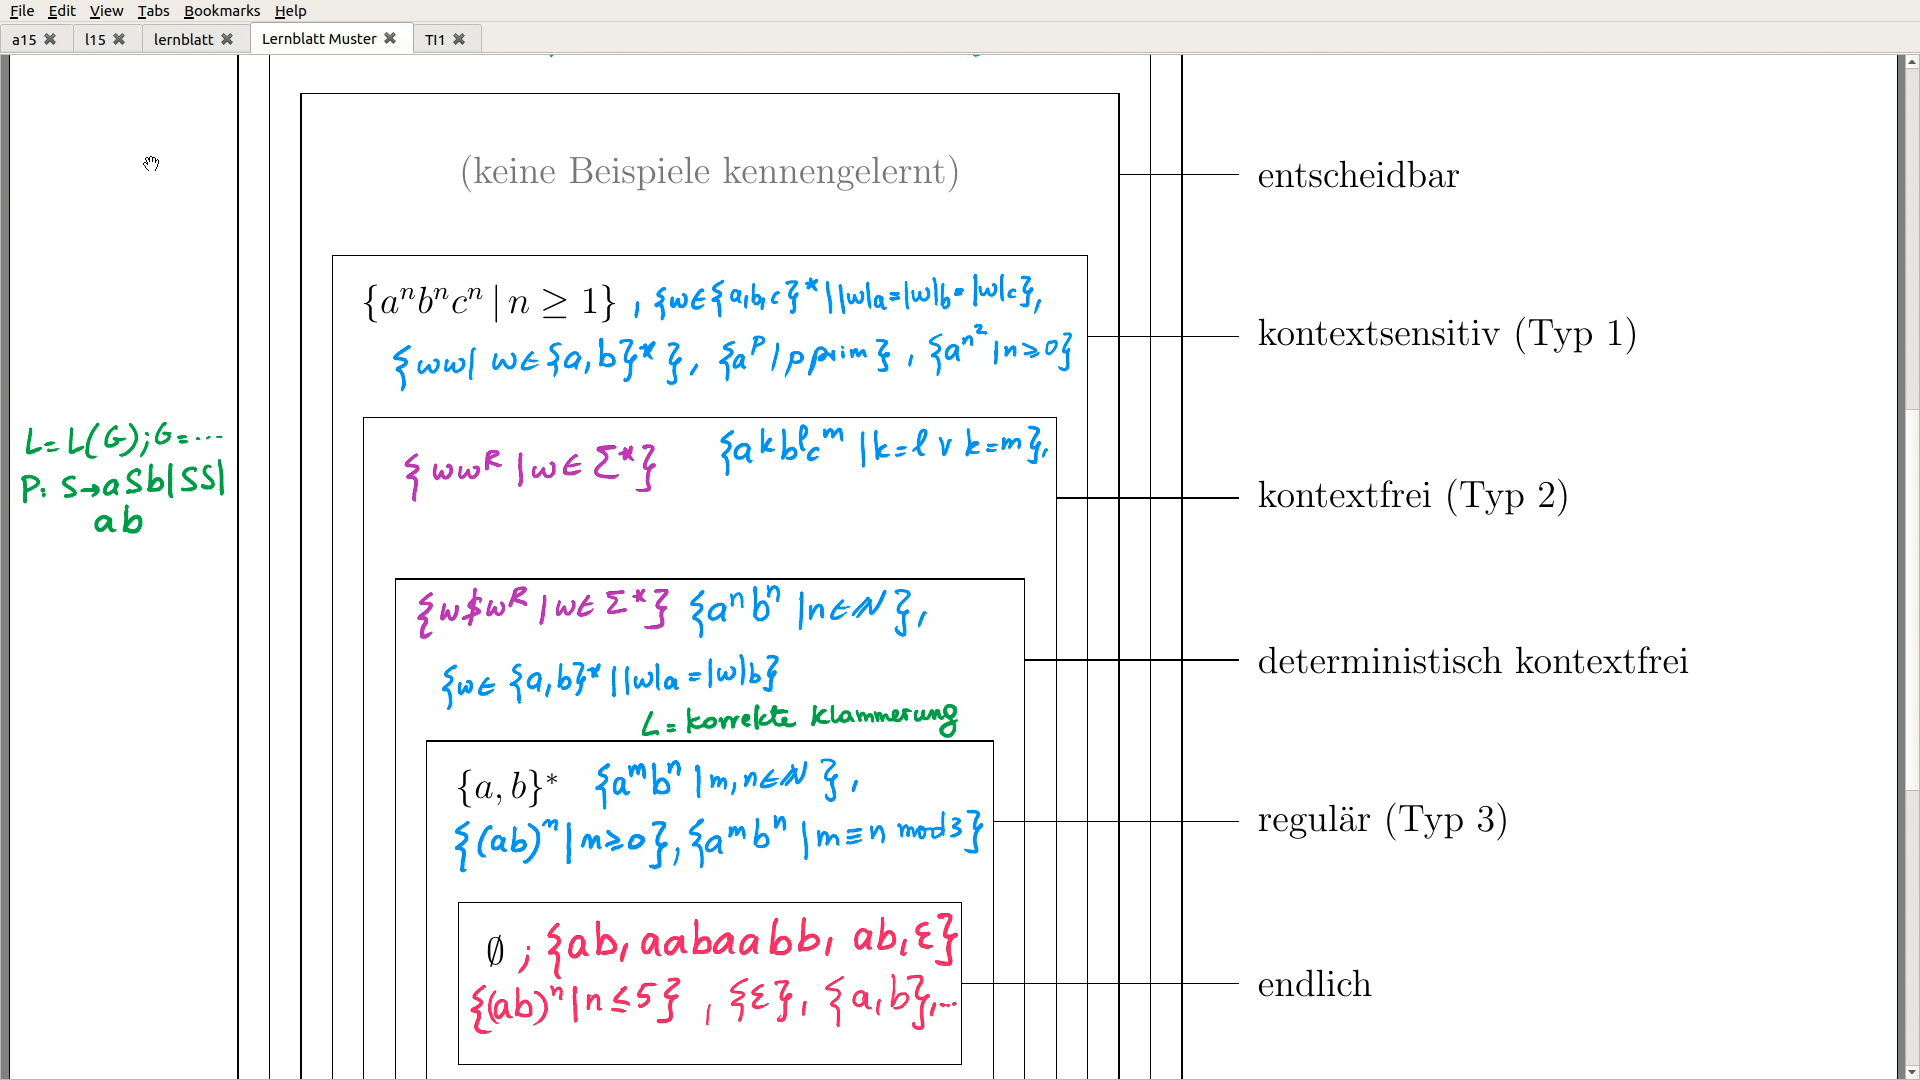
\includegraphics[width=1\textwidth]{Pictures/Chomsky.png}
				\includegraphics[width=1\textwidth]{Pictures/Verhältnisse.png}
				\end{figure}
			\item Definiton Grammatik (Ableitungen) 
			\item Abschlusseigenschaften
				\begin{figure}[!h]
				\centering
				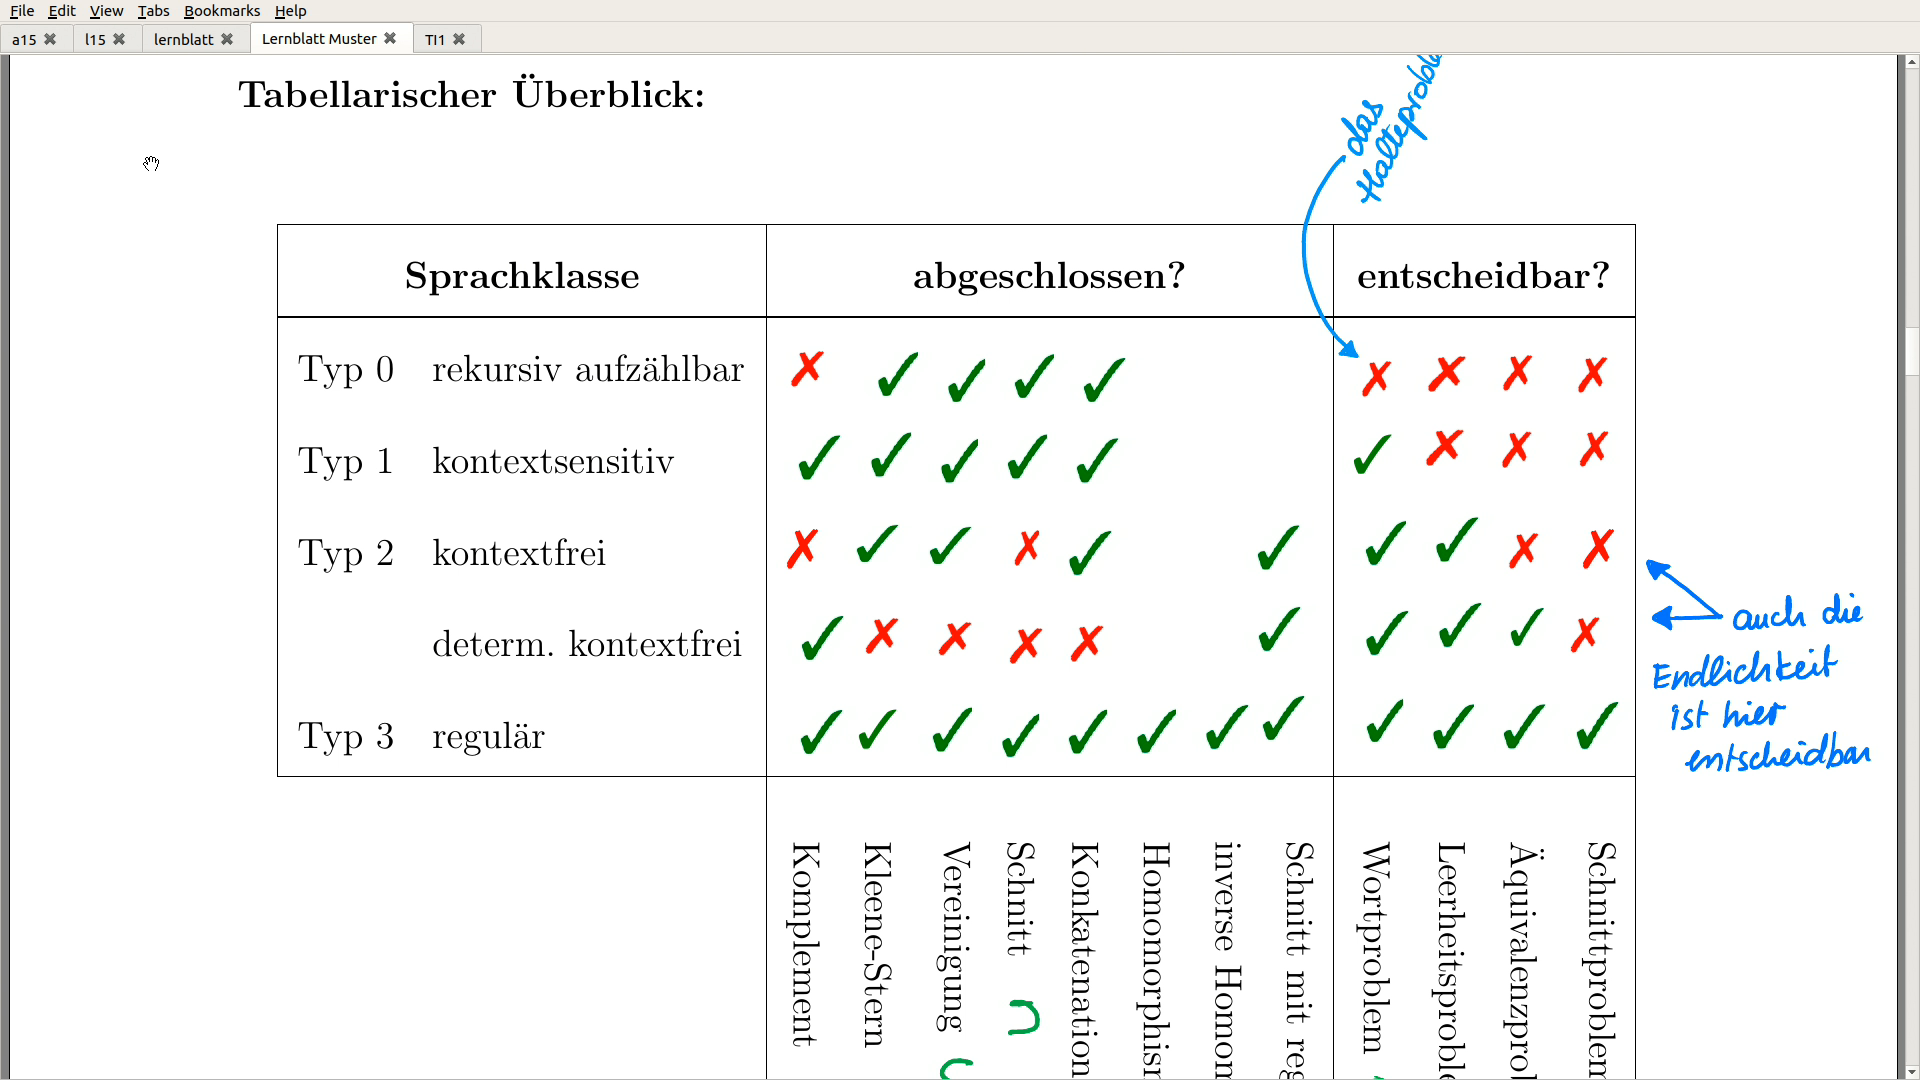
\includegraphics[width=0.9\textwidth]{Pictures/Abschlusseigenschaften.png}
				\end{figure}
			\item Typische Vertreter einer Sprache
			\item 
		\end{enumerate}
		
	\item Automaten
		\begin{enumerate}
			\item NEA und DEAS
			\item Potenzmengenkonstruktion
			\item Abschlusseigenschaften
			\item Kellerautomat (det / non det) - Konstruktion aus Sprache 
			\item Turingmaschinen 
		\end{enumerate}
		
	\item Grammatiken
		\begin{enumerate}
			\item Typ 3 Sprache - Linksableitung/Syntaxbäume
			\item Reguläre Ausdrücke
			\item Chomsky Normalform
			\item Greibach Normalform
			\item Kuroda Normalform (nur kennen)
			\item Turingmaschine zu Grammatik
			\item Typ 1 Sprachen, Kuroda-Normalform
		\end{enumerate}
		
		\item Mathematischer Teil
		\begin{enumerate}
			\item Erkennung durch Monoide 
			\item Myhill-Neurode
			\item syntaktische Monoid + Beweismethode für Typ 3
			\item allg. Beweis das eine Sprache eines best Types ist 
			\item Pumping Lemma Typ 3
			\item Pumping Lemma Typ 2
			\item Beweis einer Kongruenz (zz.: u R v $\land$ w R x $\Rightarrow$ uw R vx )
		\end{enumerate}
\end{enumerate}

\newpage

\section{Lösungen der Übungsaufgaben}
	

\end{document}
